\documentclass[a4paper,UKenglish]{oasics}
%This is a template for producing OASIcs articles.
%See oasics-manual.pdf for further information.
%for A4 paper format use option "a4paper", for US-letter use option "letterpaper"
%for british hyphenation rules use option "UKenglish", for american hyphenation rules use option "USenglish"

\usepackage{microtype}%if unwanted, comment out or use option "draft"

%\graphicspath{{./graphics/}}%helpful if your graphic files are in another directory

\bibliographystyle{plain}% the recommended bibstyle

% Author macros::begin %%%%%%%%%%%%%%%%%%%%%%%%%%%%%%%%%%%%%%%%%%%%%%%%
\title{Demand for Medical Care by the Elderly: A Nonparametric Variational Bayesian Mixture	Approach}
\titlerunning{Demand for Medical Care by the Elderly: A Nonparametric Variational Bayesian Mixture	Approach} %optional, in case that the title is too long; the running title should fit into the top page column

\author[1]{Christoph F. Kurz}
\author[1]{Rolf Holle}
\affil[1]{Helmholtz Zentrum M\"unchen,\\
  Institute of Health Economics and Health Care Management, Neuherberg, Germany\\
  \texttt{christoph.kurz@helmholtz-muenchen.de}}
%\affil[2]{Department of Informatics, Dummy College\\
%  Address, Country\\
%  \texttt{access@dummycollege.org}}
\authorrunning{C.F. Kurz}%mandatory. First: Use abbreviated first/middle names. Second (only in severe cases): Use first author plus 'et. al.'

\Copyright{John Q. Open and Joan R. Access}%mandatory. OASIcs license is "CC-BY";  http://creativecommons.org/licenses/by/3.0/

\subjclass{G.3 Probability and Statistics}% mandatory: Please choose ACM 1998 classifications from http://www.acm.org/about/class/ccs98-html . E.g., cite as "F.1.1 Models of Computation". 
\keywords{machine learning, health care utilization, Bayesian statistics}% mandatory: Please provide 1-5 keywords
% Author macros::end %%%%%%%%%%%%%%%%%%%%%%%%%%%%%%%%%%%%%%%%%%%%%%%%%

%Editor-only macros:: begin (do not touch as author)%%%%%%%%%%%%%%%%%%%%%%%%%%%%%%%%%%
\serieslogo{}%please provide filename (without suffix)
\volumeinfo%(easychair interface)
  {Billy Editor and Bill Editors}% editors
  {2}% number of editors: 1, 2, ....
  {Conference/workshop/symposium title on which this volume is based on}% event
  {1}% volume
  {1}% issue
  {1}% starting page number
\EventShortName{}
\DOI{10.4230/OASIcs.xxx.yyy.p}% to be completed by the volume editor
% Editor-only macros::end %%%%%%%%%%%%%%%%%%%%%%%%%%%%%%%%%%%%%%%%%%%%%%%

\begin{document}

\maketitle

\begin{abstract}
Outpatient care is a large share of total health care spending, making analysis of data on outpatient utilization an important part of understanding patterns and drivers of health care spending growth. Common features of outpatient utilization measures include zero-inflation, over-dispersion, and skewness, all of which complicate statistical modeling. Mixture modeling is a popular approach because it can accommodate these features of health care utilization data. In this work, we add a nonparametric clustering component to such models. Our fully Bayesian model framework allows for an unknown number of mixing components, so that the data, rather than the researcher, determine the number of mixture components. We apply the modeling framework to data on visits to physicians by elderly individuals and show that each subgroup has different characteristics that allow easy interpretation and new insights.
\end{abstract}

\section{Introduction}
Outpatient hospital services account for a large share of health care utilization and therefore of total health care spending. To understand the variation in this major component of health care expenditures, researchers have sought to identify patient subgroups with different utilization and spending patterns.

Health care resource use data are often non-negative, right-skewed, heavy-tailed, and multi-modal with a point mass at zero. Desirable analytical approaches for these data should be sufficiently powerful and flexible to accommodate all of these features.
Several authors showed that finite mixture models (FMMs) provide better model fit than single distribution generalized linear models (GLMs) and the hurdle model.~\cite{DebTrivedi, mihaylova} In addition, FMMs have two advantages: first,
they can easily handle multimodality. This may be important when the outcome distribution suggests decomposing resource use into different components.
For example, it may be necessary to fit the tail distribution separately. Second, mixture models allow us to link the prevalence of different mixture components to different covariates.~\cite{mihaylova} Generally, mixture models distinguish between different groups of users (e.g. low- and high users) and avoid the sharp dichotomy between users and non-users.

A key question in mixture models is the optimal number of components. (Note that we use component, rather than cluster, to describe the subpopulations identified by FMMs.) Too many components may overfit the data and impair model interpretation, while too few components limit the flexibility of the mixture to approximate the true underlying data structure.
The number of different user groups can be decided either ``ex-ante'' by a defined value (two or three groups are common), or ``ex-post'', i.e. chosen by model fit after calculating different models. 
While the ex-ante approach is focused on feasibility and is a one-stage decision process, ex-post approaches use information which extends beyond the time at which the actual model is prepared and involves a second decision process. Both approaches introduce a decision and model selection bias.

In this paper, we present a fully variational Bayesian (VB) hierarchical mixture model, where the optimal number of components is evaluated during model fit. This one-stage process yields both the ideal number of components and allows interpretation of each component. 
In this Bayesian nonparametric mixture model, we let the data determine both the number and the form of the local mean functions. In contrast to frequentist nonparametric regression methods, this Bayesian approach creates a model that is only as complex as the data require.~\cite{hannah} In models with a fixed, finite number of parameters, there may be misfit between the complexity of the model and the amount of data available. By contrast, Bayesian nonparametric models are less subject to over- or under-fitting: the unbounded complexity of the infinite mixture mitigates under-fitting, while the Bayesian approach of computing the full posterior over parameters mitigates over-fitting.~\cite{rasmussen}

Our model uses a Dirichlet process (DP) prior for the mixing component and comprises a fully VB regression scheme. VB is an alternative to Markov chain Monte Carlo (MCMC) sampling methods for taking a fully Bayesian approach to statistical inference over complex distributions that are difficult to directly evaluate or sample from. In particular, whereas MCMC techniques provide a numerical approximation to the exact posterior using a set of samples, VB provides a locally-optimal, exact analytical solution to an approximation of the posterior.
VB inference algorithms are usually faster than MCMC and suitable for large scale data sets, which are becoming more and more prevalent through the analysis of claims data and electronic health records.

In the following, we define a VB regression mixture model for counts and apply it on a data set to analyze outpatient health care utilization. The data set has already been used in~\cite{DebTrivedi} where Deb and Trivedi showed that a FMM with two components provides better model fit than a simple GLM. In this paper, we apply our proposed VB mixture model on the DebTrivedi data set and demonstrate that this model has good clustering and inference properties that allow new insights.

\section{Model Definition}
\subsection{Dirichlet Process Mixtures for Generalized Linear Models\label{s:dpp_models}}
The DP is a \emph{measure on measures}~\cite{blei2006} or a \emph{distribution over distributions}~\cite{sammut} parameterized by a base distribution $G_0$ and a concentration parameter $\alpha$. Each draw from a DP is a distribution that is discrete with countably infinite parameters, making this a nonparametric model.
Using a DP prior for the distribution of component means in mixture models does not require one to specify the number of components. Instead, a concentration parameter controls it implicitly.
Suppose the sample space $\Omega$ is partitioned into measurable subsets $U_1,...,U_k$. Let $\mathfrak{U}$ be the collection of all possible subsets of $\Omega$. If $G$ is a random probability measure over $(\Omega,\mathfrak{U})$ that assigns probabilities to all subsets, then $G\sim\text{DP}(\alpha, G_0)$ is a measure with property
$$
G(U_1),...,G(U_k) \sim \text{Dir}(\alpha G_0(U_1),..., \alpha G_0(U_k)).
$$
More precisely, if $\alpha>0$ and $G$ is an instantiation of a DP with base measure $G_0$, then each component $k$ has mixture weight $c_k$ sampled as follows:
\begin{align}
G&=\sum_{k=1}^{\infty}c_k \delta(\theta=\zeta_k),\quad \text{where    }\ \zeta_k \overset{\text{iid}}{\sim} G_0,\ k=1,...,\infty,\nonumber \\
v_k &= \Phi(\alpha), %\quad \alpha_k \overset{\text{iid}}{\sim} \mathcal{N}(\mu, \sigma^2) 
\quad c_k = v_k \prod_{j=1}^{k-1}(1-v_j),\quad \sum_{k=1}^{\infty}c_k=1,
\end{align}\label{eq:dp}
where $\Phi(\cdot)$ denotes the cumulative distribution function for the standard normal distribution and $\delta$ is the delta function. The base measure $G_0$ provides an initial guess at $G$, and $\alpha$ controls how close samples from the Dirichlet process are to $G_0$.
The DP serves as a nonparametric prior on the mixture components. As the $\zeta$'s are drawn from a (discrete) DP-distributed distribution, it is very likely that they will be the same in each draw. The distinct number of $\zeta$'s defines the number of components.
%This prior then serves as the parameters within another likelihood function $F$. That means, each data item $n$ chooses a component assignment $z_i\sim \text{Cat}(c)$, and then draws observations $x_n\sim F(\phi_{z_n})$. 
The representation in Equation~\ref{eq:dp} is called a \emph{stick-breaking process} and yields an infinite mixture model representation:
$$
f_\text{mix}(x|\alpha, G_0) = \sum_{k=1}^{\infty} c_k f(x|\phi_k),
$$
where $f$ is the density function with parameters $\phi_k$. Note that we define the stick-breaking process according to the probit representation~\cite{rodriguez} instead of using Beta random variables.
% * <pihive@msn.com> 2017-04-26T12:31:36.636Z:
% 
% maybe delete the stickbreaking definition from here on
% 
% ^ <pihive@msn.com> 2017-06-08T09:34:24.448Z.

%The stick-breaking representation can be illustrated as follows:
%\begin{itemize}
%	\item The initial stick has length one.
%	\item Break this stick into two portions of length $c_1=v_1$ and $(1-c_1)$. The length is generated from $\Phi(\cdot)$.
%	\item Further break the second portion $(1-c_1)$ into two portions $v_2$ and $(1-v_2)$. The length of the first portion is $v_2\cdot(1-v_1)$ and the second portions has length $(1-v_1)(1-v_2)$.
%	\item Continue to break the second portion from the previous step in this manner forever.
%\end{itemize}

In addition to the usual regression parameters, these nonparametric mixture models produce several additional parameters of interest. For each mixture component $k$, we want to estimate the relative prevalence of the mixture component in the data and parameters of the mixture component's distribution, such as the mean, variance, and regression coefficients. The mixture weights $c_k$ are the probabilities associated with each component and come directly from the  stick-breaking proportions $v_k$. The features of the mixture component are in $\phi_k$. In addition, for each observation, we want to estimate the mixture component from which it was most likely drawn, also called the component assignment.

\subsection{The Negative Binomial Regression Model}
The Negative Binomial distribution is a flexible alternative to the Poisson model for counts that accommodates over-dispersion with a longer, fatter tail.~\cite{hu}
Hilbe identified more than 12 different parameterizations of the Negative Binomial in the literature;~\cite{hilbe} here, we use the definition in~\cite{DebTrivedi}.  
%The data consists of $N$ observations $\lbrace \mathbf{x}_n, y_n \rbrace^N_{n=1}$ where $\mathbf{x}_n$ is a vector of length $D$ and $y_n$ is scalar.
For $i=1,\ldots,N$ observations and $d=1,\ldots,D$ covariates, the data comprise an $(N,D)$-dimensional covariate matrix $\mathbf{X}$ with rows $\mathbf{x}_i$ and an $N$-vector of outcomes $\mathbf{y} = (y_1,\ldots,y_N)'$. For simplicity, we omit the subscript $i$ in what follows.
The density function for the $y \sim \text{NegBin}(\mu,\psi)$ distribution is
$$
f(y) = \frac{\Gamma(y+\psi)}{\Gamma(\psi)\Gamma(y+1)}\left( \frac{\psi}{\mu+\psi} \right)^{\psi} \left( \frac{\mu}{\mu + \psi} \right)^{y},
$$
where we specify a regression model (with regression coefficients $\beta$) for the mean parameter
$$
\mu = \exp(\mathbf{x}\beta)
$$
and $\psi$ is a precision parameter.
In this specification, mean and variance are
$$
\mathbb{E}(y|\mathbf{x}) =\mu, \quad \text{Var}(y|\mathbf{x})= \mu+\psi^{-1} \mu^{2}\;,
$$
which corresponds to the NB2 model definition.~\cite{cameron}


\subsection{Variational Inference Scheme}
We assume a mixture distributions with $K$ components, each following a negative binomial regression model.
%That means, each cluster $k$ produces the output values according to the following Bayesian Negative Binomial regression model:
%$$
%y_i| \beta,\psi \sim \text{NegBin}(\exp(\mathbf{X}\mathbf{\beta}), \psi),
%$$
%with regression parameters $\beta$ and dispersion parameter $\psi$.
The data set consists of pairs $\lbrace \mathbf{x}_n, y_n \rbrace^N_{n=1}$ where $x_n$ is a vector of length $D$ and $y_n$ is scalar. Therefore, for each pair of observations %$\lbrace \mathbf{x}_n, y_n \rbrace$ 
there exists a latent variable $\mathbf{z}_n$ indicating the component assignment. The conditional distribution of the observed data vectors given the latent variables and the component parameters can be defined as:
$$
p(\mathbf{y}|\mathbf{x},\mathbf{z},\boldsymbol{\beta},\boldsymbol{\psi}) = \prod_{n=1}^N \prod_{k=1}^{K} \text{NegBin}(y_n|\boldsymbol{x}\boldsymbol{\beta},\psi)^{z_{nk}}.%,\quad \mu=X\beta.
$$
We define a Dirichlet prior over the mixing proportions $c$:
$$
p(\mathbf{c}) = \text{Dir}(\mathbf{c}|\boldsymbol{\alpha_0})
$$
and introduce a Gaussian-Wishart prior over the mean and dispersion component:
$$
p(\boldsymbol{\beta}, \boldsymbol{\psi})=\prod_{k=1}^{K}\mathcal{N}(\boldsymbol{\beta}_k|\hat{\boldsymbol{\beta}_k},\psi_k^{-1} \hat P_k^{-1}) \mathcal{W}(\psi_k|\hat \nu_k, \hat \tau_k).
$$
The joint distribution over all random variables is:
$$
p(\mathbf{y},\mathbf{x},\mathbf{z},\boldsymbol{c},\boldsymbol{\beta},\boldsymbol{\psi})=p(\mathbf{y}|\mathbf{x}, \mathbf{z},\boldsymbol \beta,\boldsymbol \psi)p(\boldsymbol{z}|\boldsymbol \beta)p(\boldsymbol{c})p(\boldsymbol{\beta}|\boldsymbol \psi)p(\boldsymbol \psi).
$$
The goal of variational inference is to optimize the parameters of a fully factorized variational distribution $q$ that minimizes the Kullback-Leibler divergence from the true intractable posterior.
The optimal $q$ maximizes the \emph{evidence lower bound} objective. Because of intractable integrals in the variational distribution
$$
q(\mathbf{z},\mathbf{c},\boldsymbol{\beta},\boldsymbol{\psi})=q(\mathbf{z})q(\mathbf{c},\boldsymbol{\beta},\boldsymbol{\psi}),
$$ We define
$$
q(\mathbf{c},\boldsymbol{\beta},\boldsymbol{\psi})= q(\mathbf{c})\prod_{k=1}^{K}q(\boldsymbol{\beta}_k,\boldsymbol{\psi}_k)= q(\mathbf{c})\prod_{k=1}^{K}q(\boldsymbol{\beta}_k,\boldsymbol\Sigma^{-1}_k),
$$
where $q(\boldsymbol{\beta}_k,\boldsymbol\Sigma^{-1}_k)=\mathcal{N}(\boldsymbol{\beta}_k,\boldsymbol\Sigma^{-1}_k).
$

The optimization problem is therefore
$$
q^*(z)=\arg\underset{q(z)\in \mathcal{D}} \min \mathrm{KL}(q(\mathbf{z},\mathbf{c},\boldsymbol{\beta},\boldsymbol{\Sigma})\|p(\mathbf{y},\mathbf{x},\mathbf{z},\boldsymbol{c},\boldsymbol{\beta},\boldsymbol{\psi})).
$$
and we solve this by memoized online variational inference as in~\cite{movi}.% using \texttt{python 2.7}.

%$$
%\begin{aligned}
% \mathcal{L}(y, x, 
% \hat{\nu}, \hat{\tau}, \hat{w}, \hat{P} )
% &= -\frac{N}{2} \log 2\pi
% \\ & \quad + \sum_{k=1}^K \sum_{d=1}^D
% c^{NW}_{1,E}(
% \hat{\nu}_k, \hat{\tau}_{k}, \hat{w}_{k}, \hat{P}_k)
% - c^{NW}_{1,E}(
% \bar{\nu}, \bar{\tau}, \bar{w}, \bar{P})
% \\
% & \quad -\frac{1}{2} \sum_{k=1}^K
% \left(
% N_k(\hat{r}) +  \bar{\nu} - \hat{\nu}_k
% \right)
% \mathbb E_q[ \log \delta_k ]
% \\
% & \quad -\frac{1}{2} \sum_{k=1}^K 
% \left(
% S_{k}^{yy}(y, \hat{r})
% + \bar{\tau} + \bar{w}\bar{P}\bar{w}
% - \hat{\tau}_k - \hat{w}_k \hat{P}_k \hat{w}_k
% \right)
% \mathbb E_q[ \delta_k ]
% \\
% & \quad + \sum_{k=1}^K
% \left(
% S_k^{yx}(x, y, \hat{r}) 
% + \bar{P} \bar{w}
% - \hat{P}_k \hat{w}_k
% \right)^T
% \mathbb E_q[ \delta_k w_k ]
% \\
% & \quad - \frac{1}{2} \sum_{k=1}^K 
% \mbox{trace}
% \left(
% \left(
% S_k^{xx^T}(x, \hat{r})
% + \bar{P}
% - \hat{P}_k
% \right)
% \mathbb E_q[ \delta_k w_k w_k^T]
% \right)
%\end{aligned}
%$$

%If $\alpha_0>0$ and $G$ is an instantiation of a Dirichlet Process (DP) with base measure $H$, $G\sim\text{DP}(\alpha_0,H)$, then each component $k$ has mixture weight $c_k$ sampled as follows:
%$$
%v_k \sim \text{Beta}(1, \alpha_0), \quad c_k = v_k \prod_{j=1}^{k-1}(1-v_j)
%$$
\section{Data}
We explore the model on the data set from Deb and Trivedi.~\cite{DebTrivedi}
It contains 4406 individuals, aged 66 and over, who are covered
by Medicare, a public insurance program. Originally obtained from the US National Medical
Expenditure Survey (NMES) for 1987/88, the data are available in the \texttt{R} package \texttt{MixAll}. 
The objective is to model the demand for medical care--as captured by the
number of physician/non-physician office and hospital outpatient visits--by the covariates
available for the patients. Here, we adopt the number of physician office visits \texttt{ofp} as the
dependent variable and use the health status variables \texttt{hosp} (number of hospital stays), \texttt{health}
(self-perceived health status), \texttt{numchron} (number of chronic conditions: cancer, heart attack, gall bladder problems, emphysema, arthritis, diabetes, other heart disease), as well as the socioeconomic
variables \texttt{gender}, \texttt{age}, \texttt{black} (race), \texttt{faminc} (family income), \texttt{school} (number of years of education), and \texttt{privins} (private insurance indicator) as regressors.

\begin{figure}[!ht]\centering
	% You can pre-specify the width of the graph:
	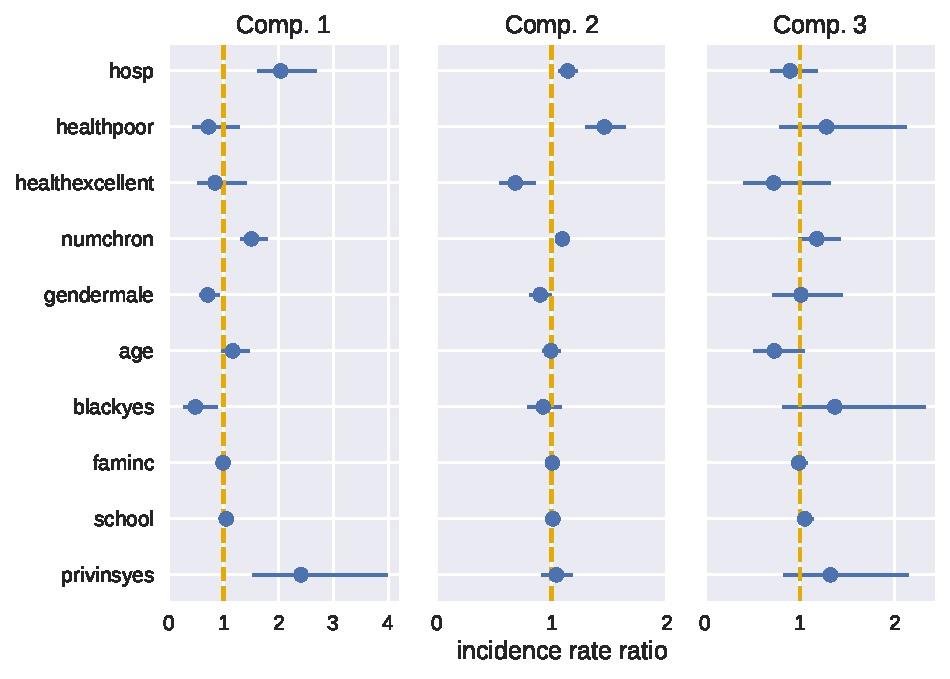
\includegraphics[width=\linewidth]{coefplot.pdf}
	% Below the figure, a caption is put, and a label is defined
	% to be used for reference to this specific figure.
	% Use labels which are very unlikely to be used by
	% other contributors; for example, use labels starting
	% with the surname of the first author.
	\caption{\label{iter} Parameter estimates for all three components on the DebTrivedi data set based on the negative binomial VB regression mixture model. Parameter estimates are presented as incidence rate ratios and 95\% high probability density intervals. Intercept is not shown. The yellow dashed line at one marks no effect.}
\end{figure}

\section{Results and Conclusion}
For the DebTrivedi data set, the VB regression mixture model finds three components.
The first component contains only 4.2\% (186/4406) of all observations and corresponds to individuals who, on average, utilize less health care, but with higher variance. The second component corresponds to the largest proportion of individuals, 62.3\%, (2745/4406) with medium health care utilization. The third component captures 33.5\% (1475/4406) of individuals, with high utilization counts and again high variance. Figure~1 presents the parameter estimates from the regression model as incidence rate ratios (IRRs). In the first component, insurance status has the largest influence with an IRR of 2.41. This means that individuals with private insurance in the first component visit the doctor more than twice as often as those without private insurance. A similar explanation can be made for the number of hospital stays in the first component: one hospital stay accounts for 2.05 times more doctor visits, on average. This effect diminishes in the other components who contain individuals with higher utilization. 

In the second component, a self perceived excellent health condition reduces the doctor visits by a factor or 0.68, while a poor health condition increases them by 1.46. This trend is slightly reduced in the third component. Most other variables show only slight effects on the number of doctor visits in the second component. In the third component, age has a protective influence on utilization, one additional year of age represents 0.73 times the utilization, on average. This seems counter-intuitive, but may be explained when comparing the age of the individuals in each cluster: Figure~2 shows that age is increasing over the components. In addition, the number of chronic diseases is also increasing in each component. That explains the highest number of doctor visits in component 3. Interestingly, the years of education also increase slightly in each component. This should be subject of further investigation as, for example, Fiscella et al.~\cite{fiscella} found that the time spent for physical examination is lower for more educated individuals.

Regarding computational speed, the VB inference method only takes 2 seconds to analyze the data set. A comparable MCMC approach took about 45 minutes on a 2016 Core i7 CPU with 32 GB RAM. This difference is mainly due to VB providing only a solution to an approximation of the posterior, while MCMC estimates the exact posterior. While we did not find great differences in the estimates in the present case, future research should investigate this difference, for example, in simulation studies.

In conclusion, the defined VB regression mixture model provides an interesting alternative with good accuracy and speed, especially suited for large data sets.

\begin{figure}[!ht]\centering
	% You can pre-specify the width of the graph:
	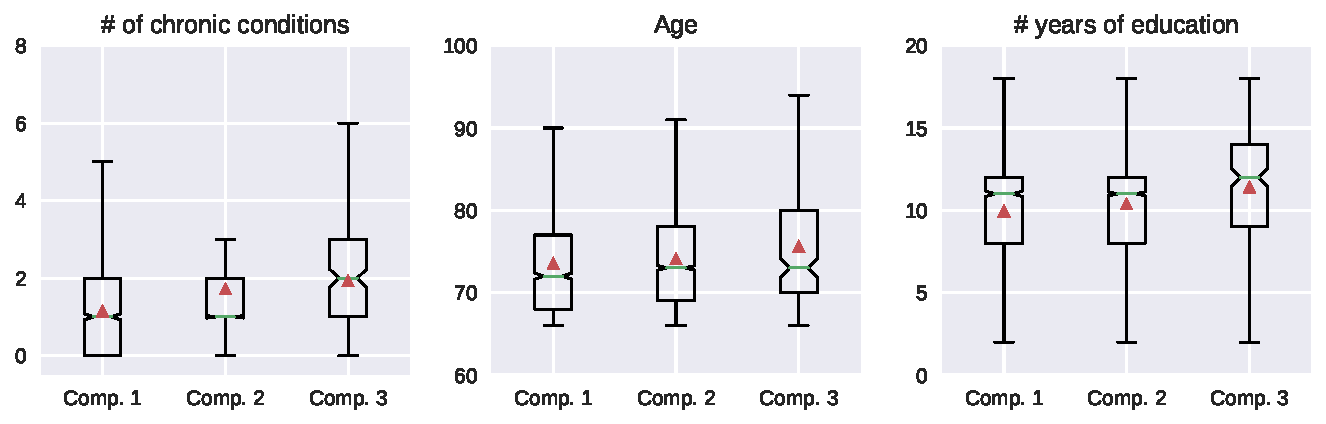
\includegraphics[width=\linewidth]{boxplot.pdf}
	% Below the figure, a caption is put, and a label is defined
	% to be used for reference to this specific figure.
	% Use labels which are very unlikely to be used by
	% other contributors; for example, use labels starting
	% with the surname of the first author.
	\caption{\label{boxplot} Boxplots for number of chronic conditions, age, and years of education for each component as modeled by the VB mixture model for the DebTrivedi data set. The red triangle marks the mean.}
\end{figure}

\subparagraph*{Acknowledgements}

We thank Laura Hatfield for improving the manuscript.

\appendix



%%
%% Bibliography
%%

%% Either use bibtex (recommended), but commented out in this sample

%\bibliography{dummybib}

%% .. or use bibitems explicitely

%\nocite{Simpson}

\begin{thebibliography}{50}
\bibitem{DebTrivedi} Partha Deb, Pravin K. Trivedi. \textsl{Demand for Medical Care by the Elderly: A Finite Mixture
Approach}, Journal of Applied Econometrics, 12, 313–336, 1997
\bibitem{mihaylova} Borislava Mihaylova, et al. \textsl{Review of statistical methods for analysing healthcare resources and costs}, Health economics 20.8, 897-916 2011.
\bibitem{hannah}Lauren A. Hannah, David M. Blei, and Warren B. Powell, \textsl{Dirichlet process mixtures of generalized linear models}, Journal of Machine Learning Research, 1923-1953, 2011.
\bibitem{rasmussen} Carl Edward Rasmussen, \textsl{The infinite Gaussian mixture model}, NIPS. Vol. 12, 1999.
\bibitem{blei2006} David M. Blei, Michael I. Jordan, et al.,\textsl{Variational inference for dirichlet process mixtures}, Bayesian
analysis, 1(1):121–143, 2006.
\bibitem{sammut} Claude Sammut and Geoffrey I. Webb, \textsl{Encyclopedia of Machine Learning}, Springer Publishing
Company, Incorporated, 1st edition, 2011.
\bibitem{rodriguez} Abel Rodriguez and David B. Dunson, \textsl{Nonparametric bayesian models through probit stick-
breaking processes}, Bayesian Analysis, 6(1), 2011.
\bibitem{hu} Mei-Chen. Hu, Martina Pavlicova, and Edward V. Nunes, \textsl{Zero-inflated and hurdle models of count data
with extra zeros: examples from an hiv-risk reduction intervention trial}, The American
journal of drug and alcohol abuse, 37(5):367–375, 2011.
\bibitem{hilbe} Joseph Hilbe, \textsl{Negative Binomial Regression}, Cambridge University Press, 2011.
\bibitem{cameron} A. Colin Cameron and Pravin K. Trivedi, \textsl{Econometric models based on count data. comparisons
and applications of some estimators and tests}, Journal of Applied Econometrics, 1(1):29–53,
1986.
\bibitem{movi} Michael C. Hughes, and Erik Sudderth, \textsl{Memoized online variational inference for Dirichlet process mixture models}, Advances in Neural Information Processing Systems, 2013.
\bibitem{fiscella} Kevin Fiscella, Meredith A. Goodwin, and Kurt C. Stange, \textsl{Does patient educational level affect office visits to family physicians?}, Journal of the National Medical Association 94.3, 157, 2002.
\end{thebibliography}


\end{document}
